\chapter[Lecture 7]{}\label{lec7}

By using unitary property of $\Gamma^{(1)}$, this becomes
\begin{equation*}
\fbox{$\sum\limits_{R}\Gamma^{(1)}(R)^{*}_{\mu'\nu'}\Gamma^{(1)}(R)_{\mu\nu}=\dfrac{h}{l_{1}}\delta_{\mu'\mu}\delta_{\nu'\nu}$}\tag{2}\label{lec7-eq2}
\end{equation*}
Combining equations \eqref{lec7-eq1} and \eqref{lec7-eq2}, we get the general form.

\section*{Geometric Interpretation}

If we have a $h$-dimensional vector space, where each axes or component is represented by the group elements $R=E$, $A_{2},A_{3}\ldots A_{h}$. [Here each vector carries three indices, representation inex, $i$; rows and column indices $\mu\nu$]. The orthogonality theorem states that all these vectors are mutually orthogonal.

In an irreducible representation of dimension $l_{i}$, no. of elements or entries are $l_{i}\times l_{i}=l_{i}^{2}$.

Since total number of elements in a group is $h$. The maximum value of $\sum l^{2}_{i}$ can be $h \Rightarrow \fbox{$\sum\limits_{\mu_{i}}l^{2}_{i}\leq h$}$.

{\bf In fact it is the equal sign that always holds.}

Since all matrix representations related to each other through unitary transformations are equivalent. There is a large degree of arbitraryness in actual form of the matrices.

We need to find a quantity which is invariant under such transformation $\to$ trace of the matrix.

$\therefore$ \ character of the $j^{\text{th}}$ representation of a set of $h$ numbers are, 
$$
\chi^{(j)}(E), \ \chi^{(j)}(A_{2})\ldots \chi^{(j)}(A_{h})
$$
$$
\chi^{(j)}(R)=T_{r}\Gamma^{(j)}(R)=\sum\limits^{k_{j}}_{\mu=1}\Gamma^{(j)}(R)_{\mu\mu}
$$
$l_{j} \to$ dimensionality of the representation.
\begin{itemize}
\item Matrix representation of all elements in a class are related by similarity transformation \fbox{$X^{-1}CX^{-1}=C$}.

Trace is invariant under such transformation.

$\therefore \ $ Character of all the elements in a class is same.

$\therefore \ $ $X^{(1)}(R)$ can be expressed as $\chi^{j}(C_{k})$ if $R\in C_{k}$ $k^{\text{th}}$ class.

\item From great orthogonality theorem:

$\chi^{(i)}(R)=\sum\limits^{l_{i}}_{\mu=1}\Gamma^{(j)}(R)_{\mu\mu}\sum\limits_{R}\Gamma^{(i)}(R)^{*}_{\mu\nu}\Gamma^{(i)}(R)_{\alpha\beta}=\dfrac{h}{l_{i}}\delta_{ij}\delta_{\mu\alpha}\delta_{\nu\beta}$ 
\begin{itemize}
\item[(i)] Put $\mu=\nu$ and $\alpha-\beta$ to get Trace.

\item[(ii)] Summing over $\mu$ and $\alpha$
$$
\Rightarrow \ \sum\limits_{R}\chi^{(1)}(R)^{*}\chi^{(J)}(R)=\dfrac{h}{l_{i}}\delta_{ij}\sum\limits_{\mu\alpha}\delta_{\mu\alpha}=h\delta_{ij}
$$
\end{itemize}
Since the character in a class is same, we can write
\begin{equation*}
\sum\limits_{k}X^{(i)}(C_{k})^{*}X^{(j)}(C_{k})N_{k}=h\delta_{ij}\tag{A}\label{lec7-eqA}
\end{equation*}
$N_{k}=$ No. of elements in $C_{k}$.

$\therefore$ \ Character of various irreducible representations form an orthogonal vector space where each axis is labeled by classes, $C_{k}$, rather than the group elements, $R$.

\item No. of orthogonal vectors is a space cannot exceed its dimensionality $\Rightarrow$ No. of irreducible representations cannot exceed the no. of classes.
\end{itemize}

\fbox{No. of irreducible representation = No. of classes}

We know \fbox{$\sum l^{2}_{i}=h$}.

$\therefore$ \ For our example group of equilateral triangle having 3 classes $C_{1}=E$, $C_{2}=A,B,C$, $C_{3}=D,F$.

We can find only one solution of dimensionalities \fbox{$2^{2}+1^{2}+1^{2}=6$}.

So, it ha $2$ one-dimensional and 1 two-dimensional irreducible representations.

\noindent
{\bf Character Table :} To form a character table, columns are labeled by classes with a prefix $N_{k}$ Rows are representations.
\begin{center}
\begin{minipage}[c]{5cm}
\begin{tabular}{>{$}r<{$}|>{$}c<{$}|>{$}c<{$}|>{$}c<{$}|>{$}c<{$}|}
\cline{2-5}
 & & C_{1} & 3C_{2} & 2C_{3}\\
\cline{2-5}
10 \text{ ---} & \Gamma^{(1)} & 1 & 1 & 1\\
\cline{2-5}
1D \text{ ---} & \Gamma^{(2)} & 1 & -1 & 1\\
\cline{2-5}
2D \text{ ---} & \Gamma^{(3)} & 2 & 0 & -1\\
\cline{2-5}
\end{tabular}
\end{minipage}
\qquad
\begin{minipage}[c]{7cm}
\begin{itemize}
\item[$\to$] Verity with explicit matrices used earlies. Simply `$i$' for each.
\end{itemize}
\end{minipage}
\end{center}

\hspace{3.5cm} $\downarrow$

Dimension, as trace of unit matrix = dimension 

$\to$ For others, use various Theorems (orthogonality....)

\bigskip

\noindent
{\bf Second orthogonality relation for characters:}

Lets form a $Q$ matrix as
\begin{align*}
Q &= \left(
\begin{matrix}
X^{(1)}(C_{1}) & X^{(1)}(C_{2}) & \ldots\\
X^{(2)}(C_{1}) & X^{(2)}(C_{2}) & \ldots\\
\ldots & \ldots & \ldots
\end{matrix}
\right)\\
\text{and}\quad Q' &= \left(
\begin{matrix}
X^{(1)}(C_{1})^{*}N_{1}/h & X^{(2)}(C_{1})^{*}N_{1}/h & \ldots\\
X^{(1)}(C_{2})^{*}N_{2}/h & X^{(2)}(C_{2})^{*}N_{2}/h & \\
\vdots & \vdots & 
\end{matrix}
\right)\\
\therefore\quad (QQ')_{ij} &= \sum\limits_{k}X^{(1)}(C_{k})_{h}X^{(j)}(C_{k})^{*}N_{k}=\delta_{ij}
\end{align*}
See \eqref{lec7-eqA} on previous page.

Two representation of same class are orthogonal.

$\therefore \ Q^{1}=Q^{-1}$ since any matrix commutes with its inverse we can write $(Q'Q)_{ij}=\delta_{ij}$.

$\therefore \ $ One can write for $k^{\text{th}}$ row in $Q^{1}$ and $l^{\text{th}}$ column in $Q$.

In the same representation character of two different class are orthogonal
\begin{equation*}
\fbox{$\sum\limits_{i}\chi^{(i)}(C_{k})^{*}X^{(i)}(C_{l})=\dfrac{h}{N_{k}}\delta_{kl}$}\tag{B}\label{lec7-eqB}
\end{equation*}
\eqref{lec7-eqA} and \eqref{lec7-eqB} are essentially same, but writing this way helps to form the character table.

\section*{Construction of character table}

\begin{itemize}
\item[(i)] No. of irreducible representation = No. of classes.

\item[(ii)] Dimensionalities can be determined from the relation
\begin{itemize}
\item[(a)] \fbox{$\sum\limits_{i}l^{2}_{i}=h$}

Since the identity element is represented by unit matrix we get

\item[(b)] \fbox{$X^{(1)}(E)=l_{i}$}

\item[(c)] Totally symmetric/identical/invariant representations $\Gamma^{(1)}$ is always represented by 1
$$
\therefore\quad \fbox{$X^{(1)}(C_{k})=1$}\quad\text{for all } k.
$$
\end{itemize}

\item Rows of the table must be orthogonal and normalized to $h$ with weighing factor $N_{k}=$ No. of elements in $C_{k}$.
$$
\therefore\quad \fbox{$\sum\limits_{k}X^{(i})(l_{k})^{*}X^{(j)}(C_{k})N_{k}=h\delta_{ij}$}
$$

\item Columns are orthogonal vectors normalized to $h/N_{k}$
$$
\therefore\quad \fbox{$\sum\limits_{i}X^{(i)}(C_{k})^{*}X^{(i)}(C_{l})=\dfrac{h}{N_{k}}\delta_{kl}$}
$$

\item Elements within $i^{\text{th}}$ row are related by
$$
\fbox{$N_{j}X^{(i)}(C_{j})N_{k}X^{(i)}(C_{k})=l_{i}\sum\limits_{l}C_{jkl}N_{l}X^{(t)}(C_{l})$}
$$
This comes from the fact that \fbox{$C_{j}C_{k}=\sum\limits_{l}C_{jkl}C_{l}$}.
\end{itemize}

\begin{proof}
We know
\begin{gather*}
X^{-1}CX=C\quad\text{for all}\quad X\in \mathfrak{g}\\
a, \fbox{$XC_{k}=C_{k}X$}\Rightarrow \fbox{$X$ (one element in $C_{k}$) = (and this element in $C_{k}$)$X$}
\end{gather*}
Now, lets assume $S_{k}=\sum\limits^{N_{k}}_{\mu=1}A_{\mu}$ 

[Sum of the matrices of all elements]

Since linear multiplication by $X$ is commutative for matrix addition, one can write
$$
\fbox{$S_{k}X=XS_{k}$}
$$
$S_{k}$ commutes with all elements.

$\therefore$ \ From Schur'c Lemma. $S_{k}=\eta_{k}E$, $\eta_{k}$ is a constant

$\therefore$ \ From $C_{j}C_{k}=\sum\limits_{l}C_{jkl}C_{l}$ one can write
\begin{equation*}
S_{j}S_{k}=\sum\limits_{l}C_{jkl}S_{l} \fbox{$\eta_{j}\eta_{k}=\sum\limits_{l}C_{jkl}\eta_{l}$}\tag{A}\label{lec7-eqA_1}
\end{equation*}
$\Tr(S_{k})=\Tr\cdot \eta_{k}E=\eta_{k}l_{i}$

$l_{i}$ dimensionality of the matrix.

again $\Tr(S_{k})=\Tr\sum\limits^{N_{k}}_{\mu=1}A_{\mu}=N_{k}X^{(i)}(C_{k})$

Thus,
$$
\fbox{$\eta_{k}=\dfrac{N_{k}X^{(i)}(C_{k})}{l_{i}}$}
$$
Substitute this in \eqref{lec7-eqA_1}.
$$
\fbox{$N_{j}X^{(i)}(C_{j})N_{k}X^{(i)}(C_{k})=l_{i}\sum\limits_{l}C_{jkl}N_{l}X^{(i)}(C_{l})$}
$$
usually rules (1), (2) and (3) are enough to form the character table.
\end{proof}

\section*{Decomposition of Reducible Representations}

Trace is sum of all diagonal elements
$$
\left(
\begin{matrix}
\Gamma^{1} & & \\
 & \Gamma^{2} & \\
 & & \Gamma^{3}
\end{matrix}
\right)
$$
$$
\therefore \ X(R)=\sum\limits_{j}a_{j}X^{(j)}(R)
$$
$a_{j}$ is No. of times $\Gamma^{(j)}$ appears in $\Gamma$.
$$
\therefore \ \sum\limits_{R}X(R)X^{(i)}(R^{*})=\sum\limits_{R}\sum\limits_{j}a_{j}X^{(j)}(R)X^{(i)}(R)^{*}=a_{i}h
$$
$\sum a_{j}X^{(j)}(R)X^{(j)}(R)^{*}=a_{j}\delta_{ij}$ (orthogonal).
$$
\therefore \ \fbox{$a_{j}=\frac{1}{h}\sum\limits_{R}X^{(j)}(R)^{*}X(R)=\frac{1}{h}\sum\limits_{k}N_{k}X^{(j)}(C_{k})X(C_{k})$}
$$
No. of times various irreducible representation appear in a reducible representation is uniquely determined by the character of the reducible representation $\to$ provided the character table of the group is known.

\section*{Regular representation}

Make a group multiplication table as
\begin{itemize}
\item[(i)] Elements along now and their inversed along column.

\item[(ii)] For element $R\to$ put $R=1$ and all others $=0$

the representation is a regular representation of $R$.
\end{itemize}

\begin{example*}
For our example group.
\begin{center}
\begin{tabular}{|>{$}c<{$}|>{$}c<{$}|>{$}c<{$}|>{$}c<{$}|>{$}c<{$}|>{$}c<{$}|>{$}c<{$}|}
\hline
 & E & A & B & C & D & F\\
\hline
E^{-1} & E & A & B & C & D & F\\
\hline
A^{-1} & A & E & D & F & B & C\\
\hline
B^{-1} & B & F & E & D & C & A\\
\hline
C^{-1} & C & D & F & E & A & B\\
\hline
D^{-1} & F & B & C & A & E & D\\
\hline
F^{-1} & D & C & A & B & F & E\\
\hline
\end{tabular}
\end{center}
\begin{figure}[H]
\centering
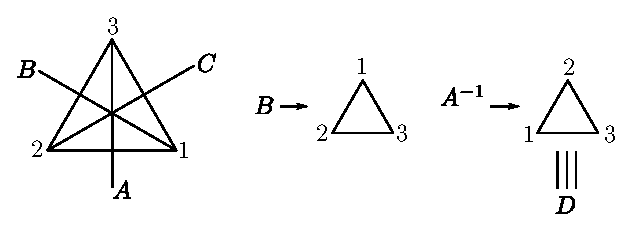
\includegraphics{images/lecture7/fig1.eps}
\end{figure}
\begin{align*}
\therefore\quad \Gamma^{\text{reg}}(A) &= 
\left(
\begin{matrix}
0 & 1 & 0 & 0 & 0 & 0\\
1 & 0 & 0 & 0 & 0 & 0\\
0 & 0 & 0 & 0 & 0 & 1\\
0 & 0 & 0 & 0 & 1 & 0\\
0 & 0 & 0 & 1 & 0 & 0\\
0 & 0 & 1 & 0 & 0 & 0
\end{matrix}
\right)\\
\therefore\quad X^{\text{[reg]}}(E) &=h\quad X^{\text{reg}}(R)=0\quad \text{for}\quad R\neq E
\end{align*}
We want to prove the following
$$
\fbox{$\Gamma^{\text{reg}}(BC)_{A^{-1}_{k}A_{i}}=\sum\limits_{A_{j}}\Gamma^{\text{reg}}(B)_{A^{-1}_{k}A_{j}}\Gamma^{\text{reg}}(C)_{A^{-1}_{j}A_{i}}$}
$$
$A_{i}$, $A_{j}$, $A_{k}\to$ are row and column indices in rearranged multiplication table.
\end{example*}

Take R.H.S.
\begin{align*}
\Gamma^{\text{reg}}(B)_{A^{-1}_{k}A_{j}} &= \left[\left.
\begin{array}{l}
1 \text{ when } A_{k^{-1}}A_{j}=B\\
0 \text{ otherwise}
\end{array}
\right|\right.\quad \text{from definition}\\
\Gamma^{\text{reg}}(C)_{A^{-1}_{j}A_{i}} &= \left[
\begin{array}{l}
1 \text{ when } A^{-1}_{j}A_{1}=C\\
=0 \text{ otherwise}
\end{array}
\right.
\end{align*}
$\therefore \ $ R.H.S. will be unity when $BC=(A_{k^{-1}}A_{j})(A_{j^{-1}}A_{i})=A_{k^{-1}}A_{i}$.

This is the left hand side.

\smallskip

$\therefore \ $ \fbox{$\Gamma^{\text{reg}}(BC)=\Gamma^{\text{reg}}(B)\Gamma^{\text{reg}}(C)$}

\smallskip

$\therefore \ \Gamma^{\text{reg}}$ forms a representation.

\smallskip

\noindent
\textbf{Celebrated Theorem:}~ A regular representation contains each irreducible representation a number of times equal to its dimensionality $\to\Gamma^{(i)}$ appears $l_{i}$ times.

\begin{proof}
We know $a_{j}=\dfrac{1}{h}\sum\limits_{R}x^{j}(R)X^{\text{reg}}(R)=\dfrac{1}{h}X^{(j)}(E)\cdot h=l_{j}$ as $X^{\text{reg}}(E)=h$ and $X^{\text{reg}}(R)=0$ for $R\neq E$ (prooved)

Now, dimensionality of $\Gamma^{\text{reg}}=h=$ sum of dimensionalities of all irreducible representation.
$$
\therefore\quad \fbox{$h=\sum\limits_{j}l_{j}\times l_{j}=\sum\limits_{j}l^{2}_{j}$}\quad\text{OR}\quad \fbox{$h=\Gamma^{\text{reg}}(E)=\sum\limits_{i}l_{i}X^{i}(E)=\sum\limits_{i}l_{i}^{2}$}
$$
\end{proof}
